%--------------------------------------------------------
% BEER PONG RULES: GAMEPLAY SECTION
%--------------------------------------------------------
\section{Gameplay}\label{sec:Gameplay}
    \subsection{Deciding Throw Order (eye-to-eye) (snake-eyes)}\label{ssec:Order}
		\begin{enumerate}[label=(\roman*)]
            \item \label{sssec:Order,ete1} Each opposition will start with a single ball each. Maintaining eye contact with the other thrower, the player will attempt to throw into the cups. 
                \begin{enumerate}[label=(\alph*), leftmargin=2cm]% Singles vs doubles
                    \item Singles: Both players get balls and throw simultaneously until one player sinks their ball and the other misses.
                    \item Doubles: The players switch off on each team each throw. The player who shit last on the team will throw eye-to-eye first.
                \end{enumerate} 
            \item \label{sssec:Order,ete_remove} During eye-to-eye, no cups are removed when balls are sunk. This includes intermediate ties. 
            \item \label{sssec:Order,ete_ties} If both balls are sunk on the same eye-to-eye throw, then nothing is decided.
                Even if one ball is sunk faster on the throw. Eye-to-eye continues until one player sinks the ball and the other does not. 
            \item \label{sssec:order,ete_2ball} Once the game of eye-to-eye is won, the winner gets possession of both balls to begin his first real throw. 
            \item \label{ssec:order,bitchcup} The bitch cup has no effect in deciding play order so a ball sunk in the bitch counts as a sunk ball. 
        \end{enumerate}
	\subsection{Throwing}\label{ssec:Throwing}
        \begin{enumerate}[label=(\roman*)]
            \item \label{sssec:Throwing,stand_behind} When throwing, players must be directly behind their pane of play of the table (see \hyperref[fig:table]{Figure \ref{fig:table}}).
                Shots taken from a standing position too far in front of the edge are void. You do not get to throw again this turn. 
            \item \label{sssec:Throwing,wrists} Wrists will always stay behind the pane of play when throwing.
                If the wrist goes over the table edge then the shot is void. You do not get to throw again this turn. 
            \item \label{sssec:Throwing,feet} Unless performing a suitable trick-shot, both feet must remain on the ground in the accepted throwing zone (see \hyperref[fig:table]{Figure \ref{fig:table}}). 
            \item \label{sssec:Throwing,bumping_table} When throwing, no player can touch/bump/move the table in order to affect the ball's outcome. 
            \item \label{sssec:Throwing,possesion} The player/team may not throw until both balls are thrown by the opponents. 
        \end{enumerate}
    \subsection{Defending}\label{ssec:Defending}
		\begin{enumerate}[label=(\roman*)]
            \item \label{sssec:Defending,blowing} When a ball hits a cup, sometimes it will spin on the rim/insides for some time.
                These balls may be ``blown" on by a player.
                Everyone blows.
                Fingering is not allowed. 
            \item \label{ssec:Defending,blowing_voids} If the ball has touched the water, it may not be blown out and the cup must be removed from play and drinking must occur for that cup. 
            \item \label{sssec:Defending,blowing_times} The player is not limited to the number of times he/she can blow. More blowing makes for a fun night... 
            \item \label{sssec:Defending,pysycedout} The defending team may do anything they want to distract the other team except for blocking the opponents view to the cups.
                Players must not cross the plane of play while doing this (see \hyperref[fig:table]{Figure \ref{fig:table}}). 
            \item \label{sssec:Defending,balltouching} Except in a bounce shot (see \ref{ssec:BounceShots}) opponents are not allowed to swipe or grab the ball until it has bounced or sank into a cup. 
        \end{enumerate}
        \footnote{The opponents may grab after the first bounce no matter where the bounce occurred.}
	\subsection{Sinking A Ball}\label{ssec:Sinking}
        \begin{enumerate}[label=(\roman*)]
            \item \label{sssec:Sinking,def} A ball is considered to be sunk when it has touched the liquid inside the cup.
                Once this has occurred, then the cup is marked for removal. 
            \item \label{sssec:Sinking,removal} Once a ball has been sunk, it is removed from the cup before the player throws their next ball.
                This is the responsibility of the defender given a reasonable time frame.
            \item \label{sssec:Sinking,non-removal} If the ball is not removed that the next ball goes into the same cup and bounces out \textit{Due to the other ball being in there}, the ball will count as sunk.
            \item \label{sssec:Sinking,cups_away} The cups are removed only after both balls are thrown in case of bomb and island shots.
            \item \label{sssec:Sinking,knockedover} A ball knocking over/knocking off and spilling its contents counts as a sunk ball. 
            \item \label{sssec:Sinking,cups_drinking} At the end of the opponent's turn, the players remove the sunk cups and take appropriate drinks.
        \end{enumerate}
	\subsection{Reracks}\label{ssec:Rerack}
		\begin{enumerate}[label=(\roman*)]
            \item \label{sssec:Rerack,number} During the game, each team can request a rerack once.
            \item \label{sssec:Rerack,notallowed} Players cannot ask for a rerack when it is not their turn, after throwing their first ball, or on balls back (including on fire).
                I.e only at the start of their go.
            \item \label{sssec:Rerack,pop_forms} Popular formations are shown in figure \ref{fig:rerack_forms}.
                You are not limited to these formations but are provided here for convenience and to avoid misunderstandings. 
            \item \label{sssec:Rerack,centering} All rerack formations should be centred on the table from side to side and two fingers from the player's edge but no maore than 4.
            \item \label{sssec:Rerack,Island} A player may not request a rerack that would give them an island cup.
            \item \label{sssec:Rerack,4cupdeep} A player may not request a rerack that puts the cups closer than the tip cup of a full rack.
                i.e. 4 cups deep towards the opponent.
            \item \label{sssec:Rerack,autoreracks} A player gets an automatic rerack at 2 and 1 cups.
                The two cups can be placed parallel or orthogonal to the pane of play.
                The last cup rerack is centred on the table.
        \end{enumerate}
        \begin{figure}[H]
            \centering
            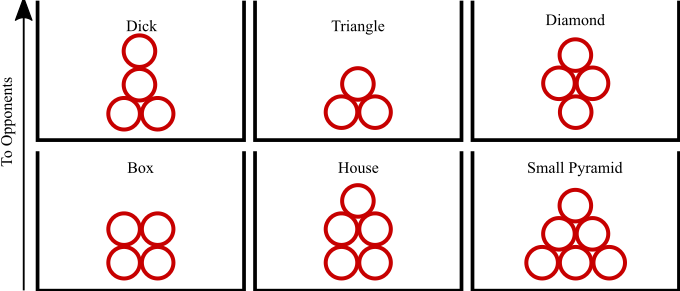
\includegraphics[width=0.75\textwidth]{rerack_formations.png}
            \caption{Popular rerack formations}
            \label{fig:rerack_forms}
        \end{figure}
	\subsection{Balls Back, On-fire, Roll Backs}\label{ssec:BallsBack}
        \noindent\textbf{Balls Back}
        \begin{enumerate}[label=(\roman*)]
            \item \label{sssec:BallsBack,bothin} If a player or team gets both balls in on the same turn, then both balls will be given back to the thrower(s) to continue the round.
                This can happen multiple times.
            \item \label{sssec:BallsBack,onfire_combine} If a player gets balls back but also onfire(see section \ref{sssec:BallsBack,onfire} to section \ref{sssec:BallsBack,onfire_calling}), The player will play the balls back shot first and continues taking the balls back following the \ref{sssec:BallsBack,bothin} Section rules.
                The player then still gets the ball back to play the on fire shots (\hyperref[ssec:BallsBack]{Section \ref{ssec:BallsBack}}) after losing balls back.
        \end{enumerate}
        \noindent\textbf{On-fire}
        \begin{enumerate}[label=(\roman*)]
            \item \label{sssec:BallsBack,onfire} If a player gets two shots sunk in a row with the same ball (1st throw and 2nd throw for singles) the player can call heating up.
                If a third is sunk with the same ball, the player is considered to be "on-fire" and will get the ball back. 
            \item \label{sssec:BallsBack,onfire_reset} All three shots do not have to occur in the same turn but must be in the same game. Remember the shots must be consecutive to be valid "on-fire" throws.
            \item \label{sssec:BallsBack,onfire_multiple} "On-fire" lasts as long as the balls are consecutively being sunk. 
            \item \label{sssec:BallsBack,onfire_calling} The player that is heating up must call heating up or they will not be on fire and get the balls back even if they get it in.
        \end{enumerate}
        \noindent\textbf{Steal Backs}
        \begin{enumerate}[label=(\roman*)]
            \item \label{sssec:BallsBack,stealback} If the balls have not touched a horizontal surface other than the table, the throwers may "steal the ball" by grabbing it before the defenders.
                They get another throw with that ball.
            \item \label{sssec:BallsBack,stealback_multi} A steal back may occur multiple times in a row.
                The player must use the non-dominant hand trick shot multiple times. This is the only exception to repeating trick shots.
            \item \label{sssec:BallsBack,stealback_redo} The first shot is void and the steal back shot will contribute to on-fire streaks and balls back double-ins.
        \end{enumerate}
	\subsection{The Bitch Cup}\label{ssec:BitchCup}
		\begin{enumerate}[label=(\roman*)]
            \item \label{sssec:BitchCup,def} The bitch cup is defined ONLY for a full rack as the centre most cup.
                See \hyperref[fig:therack]{Figure \ref{fig:therack}} for clarity. If this cup is sunk first, it does not count as sunk.
            \item \label{sssec:BitchCup,rem} If the throwers bitch cup is still in play then the throwers bitch cup is removed instead.
                If the bitch cup is already gone, the foremost cup (closest to the opponent) of the thrower is taken left to right.
            \item \label{sssec:BitchCup,song} If a bitch cup is sunk, Move Bitch by Mystikal must be played.
            \item \label{sssec:BitchCup,redemption} Called \emph{Growing a pair} a player may call redemption if they or their partner still have a ball to throw.
                If the team gets their second shot in the bitch again, no cups are removed.
            \item \label{sssec:BitchCup,redemptionFail} If the team calls redemption and gets it into a non-bitch cup, that cup is removed from the throwers rack as well.
        \end{enumerate}
	\subsection{Winning The Game/Redemption}\label{ssec:Winning}
        \begin{enumerate}[label=(\roman*)]
            \item \label{sssec:Winning,lastcup} If a team makes their last cup, the other team loses and has the chance to perform a "redemption shot"
            \item \label{sssec:Winning,redemption} The team throwing the redemption shot must make the number of shots in any cup as their opponents got into their final cup to be successful.
                This could be more than 2 as balls back is still valid on the final cup.
            \item \label{sssec:Winning,onfire} Each ball is considered to be "on fire" when starting to throw redemption shots and will follow the same rules until the thrower misses.
            \item \label{sssec:Winning,specialshot} You must not use a bonus cup to put the other team into redemption.
            \item \label{sssec:Winning,drinking} A player/team may not win unless they have drunk from all their removed cups to completion, or if playing with water cups, drinks have been appropriately drunk. 
            \item \label{sssec:Winning,death/killcups} An automatic win for the throwers can occur if a ball is sunk in a cup that was forgotten to be removed from the rack previously.
                No redemption
            \item \label{sssec:Winning,knockovers} An automatic win will occur if the opposing team knocks their entire rack off the table by accident (or on purpose?).
            \item \label{sssec:Winning,shutout} A shutout occurs when a player/team sinks there a ball in their opponent's final cup while no cups are removed from the other rack.
                There is no redemption chance for the defenders.
                The defenders must sit under the table for the next entire next match of beer pong.
            \item \label{sssec:ResidentWins} A resident of 3727 may invoke this rule and they automatically win the game.
                The other team must drink their rack or finish their drink.
            \item \label{sssec:Winning,no.Redemtions} There is no limit to the number of redemptions the players may use.
        \end{enumerate}